% ----------------------------------------
% Chap: Aufbau und Funktion des EHD-Messgeräts
% ----------------------------------------
\chapter{Aufbau und Funktion des EHD-Messgeräts}
\label{chap:aufbau_und_funktion_des_ehd_messgeraets}

Zur Schmierfilmdickenmessung wurde ein ``EHL Ultra Thin Film Measurement System'' der Firma PCS-Instrument genutzt (Abbildung \ref{fig:ehl_messgeraet}).
Es basiert auf dem Kugel-Scheibe-Modell und mit optischer Interferenz wird die Schmierfilmdicke im EHD-Kontakt ermittelt.
Durch einen leicht modifizierten Aufbau, ermöglicht das Gerät auch die Bestimmung von Reibkoeffizienten der eingesetzten Schmierstoffe.
Im Folgenden wird kurz auf die einzelnen Komponenten des EHL-Gerätes und die Modifikation im Rahmen dieser Arbeit eingegangen.

% ----------------------------------------
% Fig: EHL Prüfstand
% ----------------------------------------
\begin{figure}[htb]
    \centering
    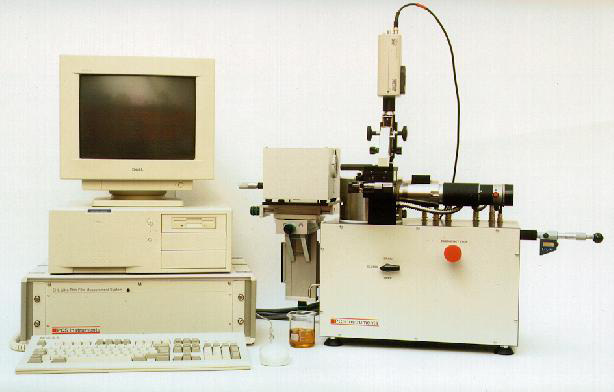
\includegraphics[width=0.8\linewidth]{./images/ehl_pruefstand.png}
    \caption{EHL-Messgerät \cite{ehl}}
    \label{fig:ehl_messgeraet}
\end{figure}

% ----------------------------------------
% Sec: PC und Elektronikeinheit
% ----------------------------------------
\section{PC und Elektronikeinheit}
\label{sec:pc_elektronikeinheit}

Zur Bedienung des Prüfstands steht einen PC zur Verfügung.
Der PC hat Windows 98 als Betriebssystem und fünf ISA-Steckkarten.
Diese Karten sind für die Ein-/Ausgabe, die Zeiterfassung, die SW-Bilderfassung sowie ADC und DAC zuständig.
Die Kommunikation mit dem Prüfstand erfolgt durch das Softwarepaket ``Ultra Thin Film EHL Measurement''.
Der PC ist mit einem Spektrometer, einem SW-Monitor und einer Elektronikeinheit verbunden.

Zu der Elektronikeinheit gehören die Motoren, die Lasteinheit sowie die Heizvorrichtung.
Außerdem ist eine Überwachungsfunktion eingebaut, die beim einem Absturz der Software oder des PC den Prüfstand abschaltet.

% ----------------------------------------
% Sec: Meschanischer Aufbau
% ----------------------------------------
\section{Mechanischer Aufbau}
\label{sec:mechanischer_aufbau}

Abbildung \ref{fig:ehl_aufbau} zeigt den Schematischen Aufbau des EHL-Prüfstands.
Das Reservoir ist bei Messungen mit Öl bis zur Hälfte der Kugel gefüllt.
Durch die Heizvorrichtung kann das Öl bis c.a \SI{150}{\degreeCelsius} temperiert werden.
% ----------------------------------------
% Fig: EHL Aufbau
% ----------------------------------------
\begin{figure}[htb]
    \centering
    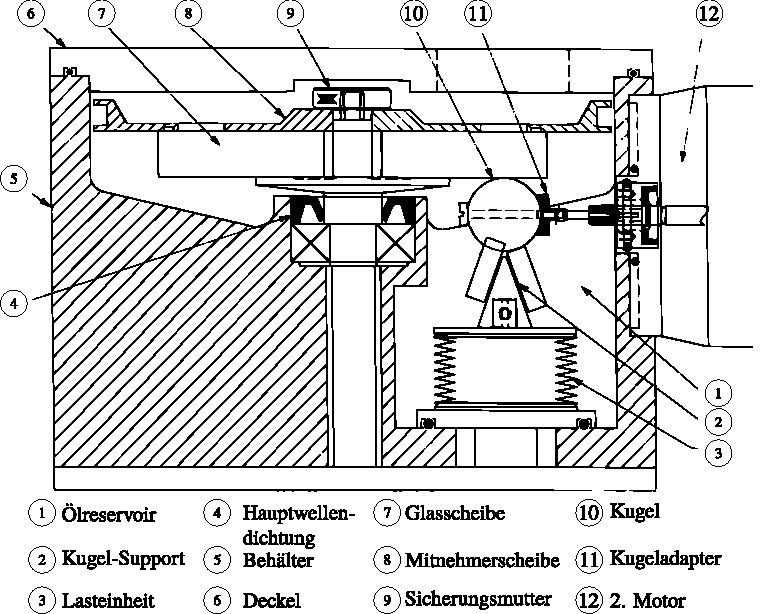
\includegraphics[width=0.8\textwidth]{./images/ehd_pruefstand_aufbau.pdf}
    \caption{Schematischer Aufbau des EHL-Prüfstands \cite{ehl}}
    \label{fig:ehl_aufbau}
\end{figure}
%
Der elastohydrodynamische Schmierfilm wird durch einen Kugel-Scheibe-Kontakt erzeugt.
Die Kugel ist hochglanzpoliert, aus 100Cr6 Stahl und hat einen Durchmesser von \SI{19.05}{\milli\meter}.
Es gibt zwei Variationen der Kugel, normal und durchgebohrt.
Über ein Kugel-Support wird die Kugel von unten von einer Lasteinheit gegen eine rotierende Glasscheibe gedrückt.
Die Last ist von \SIrange{0}{50}{\newton} wählbar und ergibt sich einen maximalen Druck von \SI{0.7}{\giga\pascal} im Kontaktpunkt.
Die Glasscheibe hat einen Durchmesser von \SI{100}{\milli\meter} und ist an der Unterseite mit einer durchlässigen Chromschicht und einer Silikatschicht zu versehen.
Es gibt insgesamt \num{21} befahrbaren Spuren ($R = 34 \rightarrow 44$ \si{\milli\meter}) auf der Scheibe durch die axiale Verschiebung des Kugel-Supports.
Ein Spurwechsel ist nötig, weil die Silikatschicht, die nicht so robust wie die Chromschicht ist, im Laufe der Zeit abgenutzt wird.

Die Glasscheibe kann von \SI[per-mode=symbol]{1}{\milli\meter\per\second} bis \SI[per-mode=symbol]{5}{\meter\per\second} durch einen Motor betrieben werden.
Ein weiterer Motor ermöglicht auch das Antreiben der Kugel.
In diesem Fall sind Versuche mit Schlupf zwischen Kugel und Scheibe innerhalb von \SIrange{0}{200}{\percent} ermöglicht.

Das originale Kugel-Support von PCS-Instrument besteht aus drei Lagern, die auf einem dreieckigen Aluminium-Klotz geschraubt werden.
Eine modifizierte Lagerung mit einstellbarer, geführte Achse von Wittek \cite{wittek_2007} steht auch zur Verfügung (Abbildung \ref{fig:kugel_support}).
% ----------------------------------------
% Fig: Kugel-Support
% ----------------------------------------
\begin{figure}[htb]
    \centering
    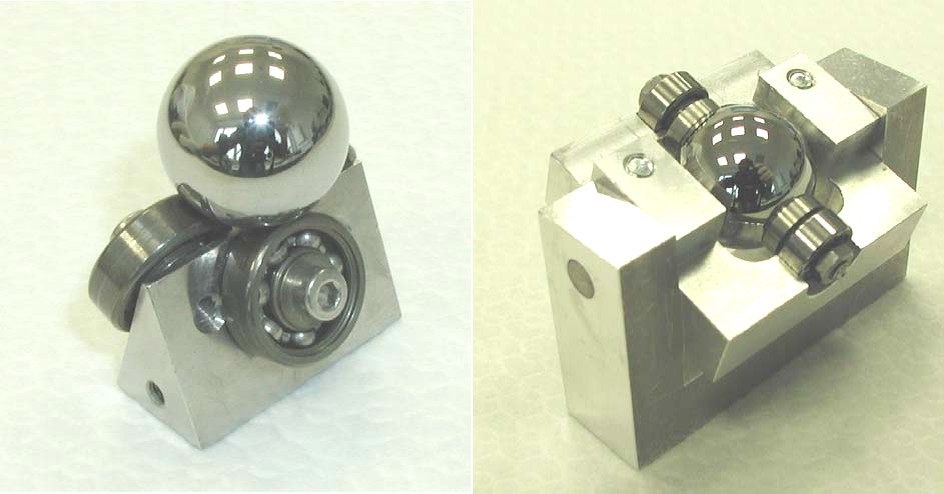
\includegraphics[width=0.6\textwidth]{./images/kugel-support_original_und_wittek.jpg}
    \caption{Originaler PCS-Support (links) und von \textit{Wittek} modifizierter Support (rechts) \cite{wittek_2007}}
    \label{fig:kugel_support}
\end{figure}
%

In Tabelle \ref{tab:ehl_specs} sind die Spezifikationen des Prüfstands von PCS zusammengefasst.

% ----------------------------------------
% Sec: Messsystem zur Schmierfilmdickemessung
% ----------------------------------------
\section{Messsystem zur Schmierfilmdickemessung}
\label{sec:messsystem_zur_schmierfilmdickemessung}

Beim EHD-Prüfstand von PCS Instrument wird die Schmierfilmdicke im Kugel-Scheibe-Kontakt mit Weißlichtinterferometrie (siehe Abschnitt \ref{sec:optische_messung_der_ehd_schmierfilmdicke}) bestimmt.
Der Kontakt wird von oben durch das Glasscheibe beleuchtet und das zurück reflektierende Bild wird von einem Spektrometer bewertet.
Die Messeinrichtung wird in Abbildung \ref{fig:ehl_messprinzip} angezeigt.
% ----------------------------------------
% Fig: EHL Messeinrichtung
% ----------------------------------------
\begin{figure}[htb]
    \centering
    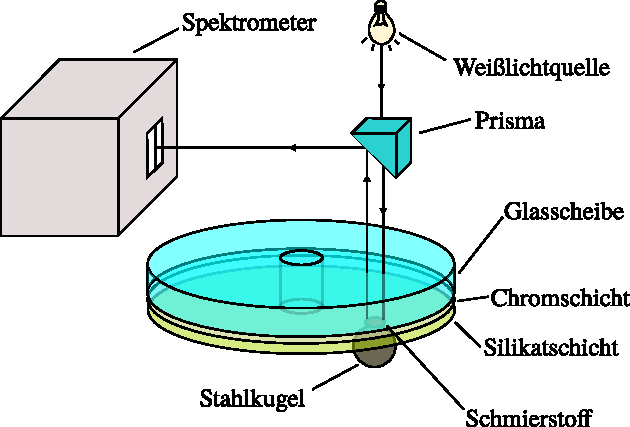
\includegraphics[]{./images/ehd_messprinzip.pdf}
    \caption{Messprinzip des EHD-Prüfstand von PCS \cite{mach_2008}}
    \label{fig:ehl_messprinzip}
\end{figure}
%

Die Glasscheibe hat nicht nur eine Chromschicht, sondern auch eine Silikatschicht (Spacer-Layer) darauf.
Diese hat die Funktion wie ein Harter-Ölfilm, der immer da ist. Das heißt, dass es auch im Stillstand Interferenzen gibt.
Interferenzmuster im Auge des Betrachters sind fabelhafte Bilder (Abbildung \ref{fig:ehl_bilder}) und aus ihrer Farben kann die Schmierfilmdicke bei bekannter Silikatschictdicke berechnet werden.
% ----------------------------------------
% Fig: EHL Interferenzbilder
% ----------------------------------------
\begin{figure}[htb]
    \centering
    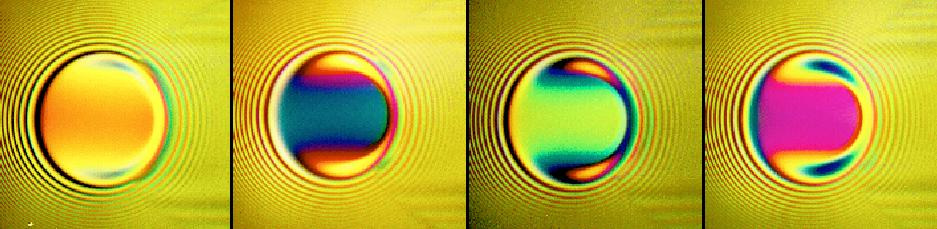
\includegraphics[width=0.8\textwidth]{./images/ehl_contact_at_increasing_speeds.png}
    \caption{Interferenzmuster eines Punktkontaktes bei zunehmenden Geschwindigkeiten \cite{ehl_broshure}}
    \label{fig:ehl_bilder}
\end{figure}
%

Da eine Auswertung der Schmierfilmdicke aus den Farben der Interferenzen durch einen Beobachter zu ungenau wäre, wird der zurück reflektierende Lichtstrahl über einen Prisma durch einen Spalt in ein Spektrometer geleitet.
Dort werden die Interferenzmuster analysiert und an einem SW-Monitor angezeigt (Abbildung \ref{fig:ehl_interferenzmuster}).

% ----------------------------------------
% Fig: EHL Beugungsmuster
% ----------------------------------------
\begin{figure}[htb]
    \centering
    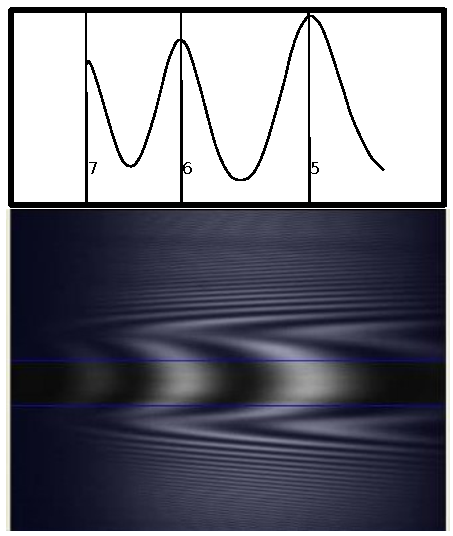
\includegraphics[]{./images/interferenzsmuster.pdf}
    \caption{Interferenzmuster im Spektrometer \cite{ehl_broshure}}
    \label{fig:ehl_interferenzmuster}
\end{figure}
%
Der senkrechte, weiße Balken im Interferenzmuster sind die Maxima, wo die konstruktive Interferenzen stattfinden und gibt dabei die Wellenlänge an.
Wandern diese Balken nach rechts, nimmt die Wellenlänge bzw. Schmierfilmdicke zu.
Mit Hilfe des Ultra-Softwarepakets kann man aus dem Interferenzmuster die genaue Schmierfilmdicke berechnet werden.

